\setlength{\footskip}{8mm}

\chapter{METHODOLOGY AND RAW MATERIAL}
\label{ch:methodology}


\textit{Some intro..}

\section{Project steps overview}

I will describe in the next paragraphs the methodology I will use for each of the steps described in Figure 3. TO BE CONTINUED

\section{Experimental design and statistical power analysis}


\addcontentsline{lot}{chapter}{Table 2 \hskip 3.55em Description of the experimental design}
\begin{center} 
  \begin{flushleft}
  \textwidth
  \addcontentsline{lot}{chapter}{Table 2.1 \hskip 3.55em Informations about animals and their origins}
  \caption{\textbf{Table 2.1 } \\
  ~ \\
  \subcaption{\textit{Informations about animals and their origins} \\
  ~ \\
  \end{flushleft} 
  \textwidth
  \begin{tabular}{ll}
    Fish population $(\mathrm{n} = 400 juveniles)$. \\
    Species = \ac{onilo}. \\
    Age = \textit{juveniles}. \\  
    Average mass of $(\mathrm{m} = X\si{\gram} \mypm X'\si{\gram})$. \\
    Secondary sexual gender: \textbf{ 100\% underwent \ac{srt}}. \\
    Origin = \textbf{Thailand}, Asian institute of technology. \\
    Strain = \textbf{Chitralada 4}. \\
    Pathogen free = \textbf{required}. \\
  \end{tabular}
\end{center}

\textbf{Detection of diseases (procedure):} Select \textbf{6-10} individuals at random, kill them, culture brain and head kidney on \ac{tsb} for detection of pathogens (\ac{a.veronii} and \ac{s.agalac}). \\

\textbf{How many groups for the vaccination?}  Create \textbf{4} groups/subsets of approx. \textbf{100-150} individuals. \\
    \textbf{4} ponds/aquariums for \textbf{10} days(Acclimatation) + \textbf{70} days(post vaccination) = \textbf{80} days. \\
  
\textbf{Methodology for flood and mucus sampling:} Select not less than \textbf{8} fish per group for \textbf{blood} and \textbf{mucus} swab every week. \\

\textbf{Challenge test:} Separate the fish in 2 sub-groups for \ac{control}, \ac{av} \textbf{monovalent}, \ac{sa} \textbf{monovalent}. In 3 sub-groups for \ac{saav} \textbf{bivalent}, as indicated below: \\
\newpage

\begin{center}
  \caption{\textbf{Table 2.2 Summary of the different groups getting vaccinated}. \\
  \\
   \begin{flushleft}
  \textwidth
  \addcontentsline{lot}{chapter}{Table 2.2 \hskip 3.55em Summary of the different groups getting vaccinated}
  \caption{\textbf{Table 2.2 } \\
  ~ \\
  \subcaption{\textit{Summary of the different groups getting vaccinated} \\
  ~ \\
  \end{flushleft} 
  \textwidth
  \begin{tabular}{ll}
    \textbf{Control} (sham vaccinated) challenged with \ac{s.agalac} = \textbf{33} fish. \\
    \textbf{Control} (sham vaccinated) challenged with \ac{a.veronii} = \textbf{33} fish. \\
    \textbf{Control} (sham vaccinated) challenged with \ac{pbs} = \textbf{33} fish. \\
    \ac{sa} \textbf{monovalent} challenged with \ac{s.agalac} = \textbf{50} fish. \\
    \ac{sa} \textbf{monovalent} challenged with \ac{pbs} = \textbf{50} fish. \\
    \ac{av} \textbf{monovalent} challenged with \ac{a.veronii} = \textbf{50} fish. \\
    \ac{av} \textbf{monovalent} challenged with \ac{pbs} = \textbf{50} fish. \\
    \ac{saav} \textbf{bivalent} challenged with \ac{s.agalac} = \textbf{33} fish. \\
    \ac{saav} \textbf{bivalent} challenged with \ac{a.veronii} = \textbf{33} fish. \\
    \ac{saav} \textbf{bivalent} challenged with \ac{pbs} = \textbf{33} fish. \\
  \end{tabular}
\end{center}
    
\textbf{Statistical power analysis:}  It is possible to create an artificial population of each group composed of 20 000 sampling with replacement and use the Central limit theorem to deduce the Standard error of the means and infer our vaccine efficiency for all the juveniles Chitralada 4 in the world (main population) with 95\% confidence using an approximation of the Standard deviation.

\section{Methodology for pond preparation and fish stocking}

\newpage

\section{Methodology for bacterial culture and bacterial preparation}

\beginfigure
  \begin{center}
  \begin{flushleft}
  \caption{\textbf{Figure 3: Schema of an antibiogram}}
  \end{flushleft} \\
  \\
  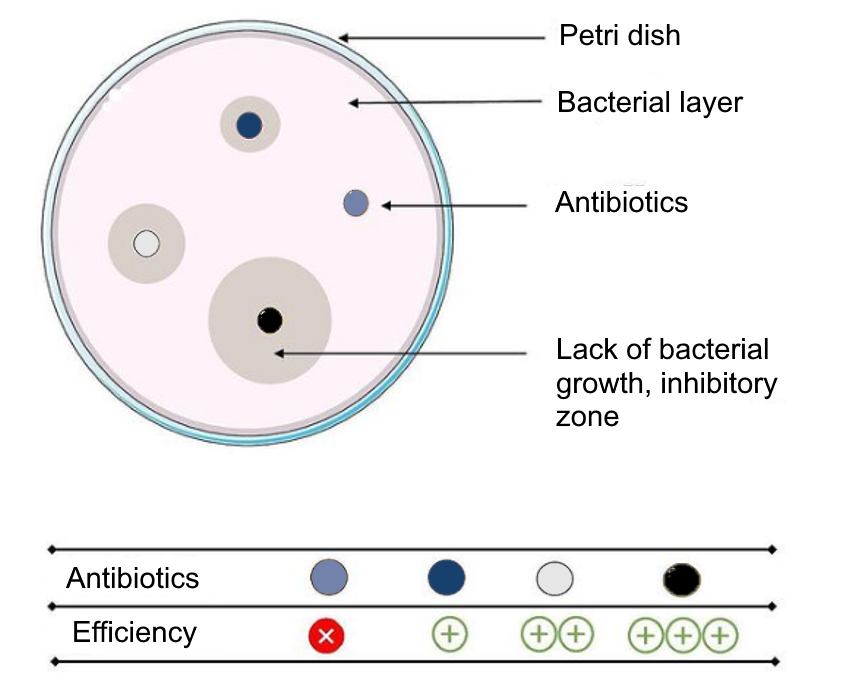
\includegraphics[width=0.8\textwidth, height=0.8\textheight, 
                 keepaspectratio]{figures/Figure3a.png}
  \label{Figure 3: Schema of an antibiogram (general principle)}
  \addcontentsline{lof}{chapter}{Figure 3 \hskip 3.55em Schema of an antibiogram (general principle)}
  \endfigure
  \end{center}


\subsection{For \ac{s.agalac}}

Antibiogram \ac{s.agalac}: 

\subsection{For \ac{a.veronii}}

Antibiogram \ac{a.veronii}: 


\section{Methodology for preparation of formalin killed vaccines (FKVs)}

Volume to inject  ${100\si{\micro\liter}\ac{ip} / fish}$

\section{Methodology for vaccine administration in fish and monitoring of fish health during bacterial challenge test}

\section{Methodology for fish sera and mucus extraction}

\section{Methodology for \ac{elisa} assays for specific \ac{igm}, \ac{igt} titrations}

\ac{elisa} is an enzyme-linked immunosorbent assay "for the presence of antibodies, antigens", proteins and glycoproteins in biological samples. \ac{elisa} technique is widely used for rapid diagnostic tests such as the diagnosis of HIV infection, pregnancy tests or the detection of food allergens.

The principle of this technique is based on the use of an enzyme conjugated to an antibody which by reacting with a colorless substrate gives a colored reaction product and which is therefore detectable. This is called a chromogenic substrate. Different enzymes are used for \ac{elisa} tests including alkaline phosphatase, \ac{hrp} or beta-galactosidase.

The \ac{elisa} assay will give information on the \ac{ab} titer of the fish, \ac{igm} and \ac{igt} respectively will be targeted in the assay.

\section{Methodology for \ac{rtpcr}}

The reference genes for the \ac{rtpcr} of \ac{onilo} are genes ubiquitously and constitutively expressed in the animal. They are also well known as "house-keeping" genes/mRNAs. (see below). 

\beginfigure
  \begin{center}
  \begin{flushleft}
  \caption{\textbf{Figure 4: Reference genes used in RT-PCR technique for Tilapia}
  \subcaption{\textit{Credits:\url{http://dx.doi.org/10.1016/j.gene.2013.06.013}}}
  \end{flushleft} \\
  \\
  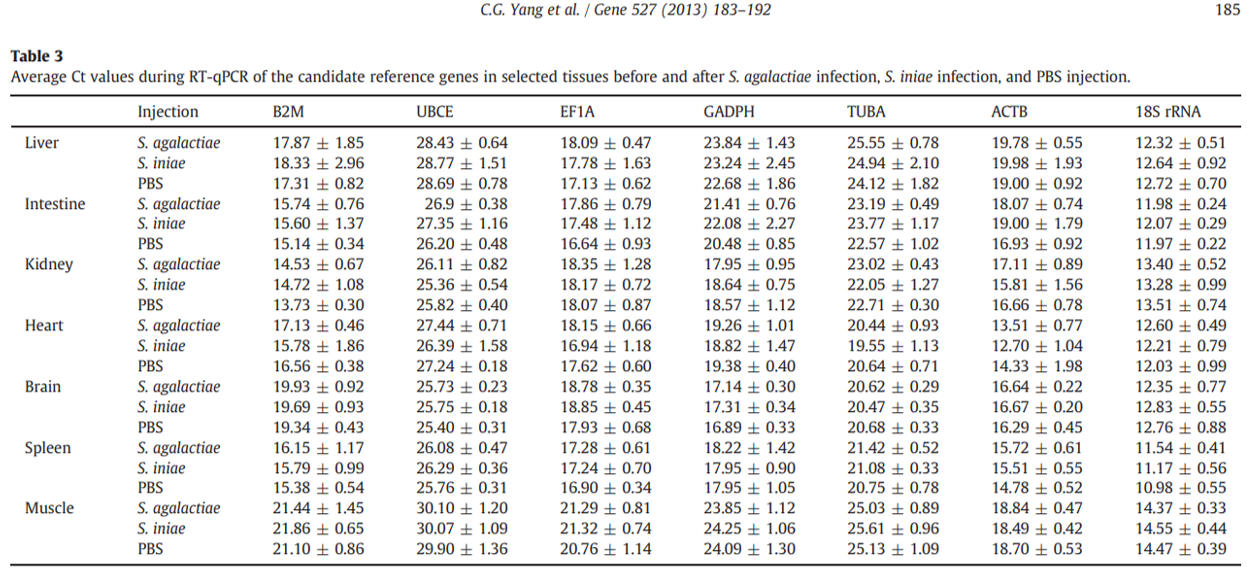
\includegraphics[width=\textwidth, height=\textheight, 
                 keepaspectratio]{figures/FigurePCR.png}
  \label{Reference genes used in RT-PCR technique for Tilapia}
  \addcontentsline{lof}{chapter}{Figure 4 \hskip 3.55em Reference genes used in RT-PCR technique for Tilapia}
  \endfigure
  \end{center}


\section{Methodology for antibody agglutination titration} 

\section{Methodology for data curation and result analysis}

ANOVA 1 way, + post hoc test tukey with signif not more than 0.05, Rstudio

\section{List of raw material}

\subsection{Price of raw material}

\section{Chapter Summary}


\FloatBarrier
